\documentclass[aps,prd,twocolumn,superscriptaddress]{revtex4-1}
% Intended to be built with pdflatex, using the REVTEX 4.1 package.
% Template taken from FermiLab APS Jouranl template.

% packages
\usepackage{amssymb}              % for \gtrsim ...
\usepackage{amsmath}              % for \text, align, split ...
\usepackage{color}                % for colorful margin notes
\usepackage[mathscr]{euscript}    % for \mathscr
\usepackage{graphicx}             % for \includegraphics
\usepackage{hyperref}             % for \url and \href
\usepackage{listings}             % for typesetting code with \lstinline
\usepackage{tabularx}             % for tabularx

% commands/initialization
\hyphenation{ALPGEN} % avoid incorrect hyphenation
\hyphenation{EVTGEN} % ''
\hyphenation{PYTHIA} % ''
\lstset{basicstyle=\ttfamily} % define \lstinline for inline code snippet

\newcommand{\todo}[1]{\marginpar{\tiny{\textcolor{red}{#1}}}}
%\renewcommand\todo[1]{} % if you wish to hide all todo notes

% *******************************************************************************
\begin{document}

\widetext
\leftline{Compiled \today}
\leftline{To be submitted to PRD}

\title{Scattering and Pair Processes in General Relativistic Ray Tracing for Neutrinos}
\todo{you sure about including all processes?}

\author{M.\ Brett Deaton}
\affiliation{Joint Institute for Nuclear Astrophysics,
  Michigan State University, East Lansing, MI 48824, USA}
\affiliation{Department of Physics,
  North Carolina State University, Raleigh, NC 27695, USA}
\email{mbdeaton@ncsu.edu}

\author{Jerred Jesse}
\affiliation{Department of Physics \& Astronomy,
  Washington State University, Pullman, WA 99164, USA}

\author{Evan O'Connor}
\affiliation{Department of Physics,
  North Carolina State University, Raleigh, NC 27695, USA}

\author{Francois Foucart}
\affiliation{Lawrence Berkeley National Laboratory,
  1 Cyclotron Rd., Berkeley, CA 94720, USA}

\author{Andy Bohn}
\affiliation{Center for Radiophysics and Space Research,
  Cornell University, Ithaca, NY 14853, USA}

\author{Matthew D.\ Duez}
\affiliation{Department of Physics \& Astronomy,
  Washington State University, Pullman, WA 99164, USA}

\author{G.\ C.\ McLaughlin}
\affiliation{Department of Physics,
  North Carolina State University, Raleigh, NC 27695, USA}

% *******************************************************************************

\begin{abstract}
  We present a covariant ray tracing algorithm for computing high-resolution
  neutrino distributions in general numerical spacetimes with hydrodynamical
  sources.
  Our formulation treats scattering and pair processes
  by incorporating estimates of the background neutrino fields.
  These background fields may be taken from a low-order moment simulation,
  be supplied analytically in simple cases,
  or be ignored entirely, in which case the method
  reduces to a standard state-of-the-art ray tracing formulation.
  It handles radiation in regimes spanning optically thick to optically thin.
  We test the new code, highlight its strengths and weaknesses, and
  apply it to simulations of neutron star mergers to
  1) compute neutrino fluxes as a function of energy and emission angle, and
  2) compute the radiation pressure tensor in the funnel of the disk,
  demonstrating a way to improve the closure relations used in the truncated
  moment formalism.
\end{abstract}

\maketitle

\section{Introduction}
Neutrinos are one of the dominant energy transport phenomena at play in
neutron star mergers, heating, cooling, and pushing the disrupted nuclear
matter.
In addition, they change the composition of the matter via charged current
interactions.
Because neutrinos scatter over length scales both large and small with
respect to fluid scales, accurate models require a neutrino treatment that
respects the freedom of neutrino distribution functions to vary
drastically from thermodynamic equilibrium.

This is a challenging task in the environment of a merger,
which generally lacks any spatial symmetries so that fully general
seven-dimensional solutions to the Boltzmann Equation are not feasible.
Leakage approximations
\citep{deat2013-leakage, pere2016-asl, radi2016-dynamical, ?}
capture the qualitative effects of neutrinos on the matter, but
produce limited information about the neutrino field itself.
Monte Carlo methods \citep{abdi2012-monte_carlo, rich2015-monte_carlo}
suffer from noise.
\todo{discuss mc more clearly}
The state of the art today employs a truncated moment formalism
\citep{shib2011-truncated_moment, fouc2015-m1_nsbh, fouc2016-m1_nsns,
  just2015-m1_code, ?},
evolving the zeroth- and first-angular moments of the distribution function
(the energy density and flux respectively) representing the zeroth-energy moment
of the radiation field (the total energy).
Recently, \cite{fouc2016-m1_evolve_n} have expanded their code to also evolve
the number densities of neutrinos, providing an estimate of the average neutrino
energies in addition to their totals.
But with only two angular moments and one energy moment, the distribution
function has very limited angular and spectral information.

\subsubsection*{What physics problems do we want to address?}
But many interesting unsolved problems require an accurate model of the neutrino
spectra and angular distributions.
With a model of the neutrino emission from a merger we can
1) examine neutrino effects on the nucleosynthesis of the ejected material
\citep{surm2011-nickel_56, robe2016-sph_nu_nucleo},
2) explore the rich flavor oscillation physics likely to occur
\citep{malk2012-mnr_1, malk2015-mnr_2, malk2016-mnr_3, zhu2016-mnr_nsns_remnant,
  vaan2016-uncovering_mnr},
3) improve closure relations used in truncated moment schemes
\citep{ramp2002-truncated_moment, shib2011-truncated_moment,
  card2013-truncated_moment, fouc2015-m1_nsbh, ocon2015-gr1d_with_nu}, and
4) study possible jet formation due to neutrino annihilation
\citep{ruff1999-nunubar_nsns, asan2000-nunubar, birk2007-nunubar,
  hari2010-gr_nunubar_collapsar, zala2011-nunubar, leng2014-nunubar}.

\subsubsection*{Why ray tracing?}
In this work we present a ray tracing method to compute neutrino distribution
functions from state-of-the-art general relativistic radiation
hydrodynamics simulations.
We choose ray tracing because it is conceptually simple, numerically cheap,
and easily extends to high resolution in energy and angle.

With a ray tracing method we approach radiation transport from the perspective
of a single observer at a spacetime event $x_o^\alpha$.
Our goal is to compute the distribution function
$f^{\nu_\sigma}(x_o^\alpha;p_\beta)$, or the amount of neutrino radiation
with momentum $p_\beta$ impinging on $x_o^\alpha$;
$\nu_\sigma$ labels this distribution function as describing one of the
six species of neutrinos or antineutrinos.
To do so we trace a geodesic trajectory in the backwards direction
$-p_\beta$ to sample the incoming radiation along that line of sight.
By tracing a family of rays intersecting $x_o^\alpha$ we build up a
picture of the distribution function there.
And by sampling many observation points we construct a global picture
of $f^{\nu_\sigma}(x^\alpha;p_\beta)$.

The ray tracing framework
is conceptually simple because it interprets the equation of radiation
transport (Eqn.~\ref{eqn:boltzmann})
as a one-dimensional ordinary differential equation,
it is numerically cheap because it confines computations of
$f^{\nu_\sigma}(x_o^\alpha;p_\beta)$ to the past light-cone of $x_o^\alpha$,
and it easily extends to high resolution in energy and angle by simply
increasing the number of rays sampled.

\subsubsection*{What is new and better about this ray tracing formulation?}
Several ray tracing formulations for radiation transport already exist.
Most formulations assume an analytic spacetime metric
\citep{birk2007-nunubar, hari2010-gr_nunubar_collapsar, kova2011-gr_ray_tracing}.
And many make the simplifying assumption of blackbody emission from a
neutrinosurface \citep{birk2007-nunubar, kova2011-gr_ray_tracing}.
Current state-of-the-art ray tracing formulations avoid the assumption of
blackbody spectra by integrating a local emissivity along each geodesic
(e.g. \cite{hari2010-gr_nunubar_collapsar} for neutrinos and
\cite{youn2012-gr_radiative_transfer} for photons).
But no formulations to date account for the important scattering and pair
processes outlined in Tab.~\ref{tab:neutrino_processes}.

We build upon existing ray tracing formulations
by eschewing any assumptions about the spacetime geometry
and by including scattering and pair processes in the integration along each
geodesic.
To incorporate these neutrino processes in our method, we employ
estimates of the first two angular moments of the distribution function
computed in a truncated moment scheme (formulated by
\cite{thor1981-truncated_moment, shib2011-truncated_moment}
and applied e.g. in \cite{ramp2002-truncated_moment,
  card2013-truncated_moment, fouc2015-m1_nsbh, ocon2015-gr1d_with_nu}).
If the first two angular moments are not available either from
a truncated moment evolution or a trustworthy analytical estimate,
our method reduces to the current state-of-the-art ray tracing method,
neglecting scattering and pair processes.

\subsubsection*{Why does a covariant formulation matter?}
We formulate our ray tracing equations covariantly---free from
assumptions about the spacetime geometry or coordinates. This is essential
because we want to apply the method as a postprocessing step using
time snapshots of data computed from general relativistic evolutions.
The spacetime represented in these snapshots is not analytic (i.e. Kerr).
And even in configurations that are described well by the Kerr metric
(e.g. a low-mass disk around a massive black hole),
the evolution coordinates are unlikely to present the metric in
a familiar analytic form.
This is because integrating the Einstein Equations often requires complicated,
time-dependent guage conditions
\citep{lind2007-gen_harmonic, fouc2013-compactness_and_spin}.

\subsubsection*{Why do scattering and pair processes matter?}
Inelastic scattering and pair processes introduce significant changes to
a spectrum,
\todo{clarify these terms}
\todo{justify these statements}
and elastic scattering can signicantly modify neutrino
distributions in angle, and dilute the emitted spectrum over a larger emitting
surface \citep{pere2016-asl}, especially for heavy-lepton neutrinos.
Any phenomena that involve neutrino-neutrino interactions (neutrino oscillations,
and neutrino-antineutrino annihilation) can depend sensitively on the angular
distribution.
And spectral changes can strongly affect the nucleosynthesis
occuring in the ejected and irradiated material.
\todo{justify these statements}

\subsubsection*{In what ways is this method limited?}
Ray tracing is ideally suited to problems requiring detailed knowledge of
radiation distribution functions over small regions of spacetime:
for example along a matter or radiation trajectory,
or over a small volume outside a source.
But the method becomes computationally burdensome when the inquiry extends
to large volumes of spacetime.

More fundamentally, though, ray tracing is limited by its naive
treatment of the Boltzmann Equation (Eqn.~\ref{eqn:boltzmann}),
a treatment which essentially decouples different neutrino momenta and species.
\todo{clarify how momenta are decoupled}
In this paper we outwit this limitation by incorporating coupling
terms that depend on either previously-evolved or analytical
estimates of the neutrino fields.
We also retain the freedom to drop the coupling terms, in which case our method
becomes similar to existing state-of-the-art ray tracing methods.
Our method is not a standalone radiation transport scheme,
but serves as the final component of a hybrid scheme,
piggy-backing on a lower-order radiation transport method as a
post-processing step.

\subsection{Outline}
In Sec.~\ref{sec:formulation} we derive the ray tracing equations from the
Boltzmann Equation and describe our numerical scheme.
In Sec.~\ref{sec:tests} we present some tests of the code.
In Sec.~\ref{sec:applications} we present two applications:
neutrino spectra as a function of observer's angle, and
a variable closure relation for a truncated moment formalism.
We present both applications in the dynamical environments following the merger
of a neutron star--neutron star and a black hole--neutron star binary.

Greek tensor indices ($\alpha, \beta, ...$) range over all four coordinates,
whereas Latin indices ($i, j, ...$) range over the spatial coordinates 1--3.
We use naturalized units in which $\hbar=c=1$.
And for the remainder of this article we suppress the neutrino species label
$\nu_\sigma$ since the formulation is general to any species.

\section{Ray tracing formulation}
\label{sec:formulation}
The neutrino distribution function, $f(x^\alpha; p_\beta)$ is an invariant
quantity counting the number of neutrinos in a given six-volume of phase
space centered on $(x^\alpha,p_\beta)$.
The phase space volume elements are defined with respect to a fiducial
observer passing through event $x^\alpha$ with velocity $u^\alpha$:
\begin{align}
  \label{eqn:dV}
  dV & \equiv \sqrt{-\psi} \, dx \, dy \, dz \, u^t \\
  \label{eqn:dP}
  dP & \equiv \frac{1}{\sqrt{-\psi}} \, dp_x \, dp_y \, dp_z \,
  \frac{1}{p^t}(-p_\mu u^\mu),
\end{align}
where $\psi$ represents the determinant of the spacetime metric,
the index $t$ indicates the time-component of the given four-vector, and
\begin{equation}
  \label{eqn:varepsilon}
  \varepsilon \equiv -p_\mu u^\mu
\end{equation}
is the neutrino energy measured by our observer.
The number of particles in a given six-volume is
$dN=g\,f\,dV\,dP/(2\pi)^3$,
where $g$ counts the number of spin states accessible to the
particles ($g=1$ for neutrinos), and $f$ is the distribution function.
Each of $dN$, $dV$, $dP$, and $f$ are spacetime invariants
\citep{debb2009-gr_boltzmann_1, debb2009-gr_boltzmann_2, lind1966-gr_boltzmann}.

We may decompose the neutrino momentum like
\begin{equation}
  \label{eqn:def_momentum}
  p_\beta = \varepsilon (u_\beta + \ell_\beta),
\end{equation}
with $\ell_\beta$ the direction normal subject to the constraints
$u^\alpha \ell_\alpha = 0$ and $\ell^\alpha \ell_\alpha=1$.
With this decompositon we can write the arguments to the distribution function
$f(x^\alpha;\varepsilon,\ell_\beta)$.

Because $\ell_\beta$ is subject to two constraints
(normalization and orthogonality to the observer's velocity)
it has two degrees of freedom; we make this explicit by defining its
spatial components with respect to spherical polar angles
\begin{equation}
  \label{eqn:def_direction}
  \ell_\alpha :=
  q (s,\sin\upsilon_1\cos\upsilon_2,\sin\upsilon_1\sin\upsilon_2,\cos\upsilon_1),
\end{equation}
with $q$ and $s$ functions of $\upsilon_1$ and $\upsilon_2$.
Now our symbol for the distribution function,
$f(x^\alpha;\varepsilon,\upsilon_1,\upsilon_2)$,
makes manifest its seven independent arguments.

\subsection{Boltzmann Equation}
\label{ssec:boltzmann}
Neutrino radiation obeys the relativistic Boltzmann Equation
\todo{point out limit of QKEs}
\begin{equation}
  \label{eqn:boltzmann}
  \frac{d}{d\lambda}f(x^\alpha;\varepsilon,\upsilon_1,\upsilon_2) = C[f],
\end{equation}
where $\frac{d}{d\lambda}$ denotes a derivative with respect to the affine
parameter defining the neutrino momentum (Eqn.~\ref{eqn:geodesic_x})
and $C[f]$ is the source term arising from interactions with the medium.
The source term varies over phase space $(x^\alpha,p_\beta)$,
and depends locally on the distribution function $f$
and nonlocally on the distribution function of this neutrino and its
antiparticle at different momenta, $f'$ and $\bar{f}'$.
For clarity we symbolize all of these dependencies with the shorthand $C[f]$.
The various neutrino interactions contributing to $C[f]$ are detailed in
App.~\ref{sec:source_terms}.

We make the right hand side of Eqn.~\ref{eqn:boltzmann} explicit by writing
the source term linear in $f$:
\begin{equation}
  \label{eqn:boltzmann_linear}
  \frac{d}{d\lambda}f =
  \mathscr{E}^* - \mathscr{K}^* f,
\end{equation}
where we have introduced
$\mathscr{E}^*$, the invariant total emissivity, and
$\mathscr{K}^*$, the invariant total opacity,
and for simplicity we have suppressed the arguments of $f$.
These coefficients are derived by considering Fermi-blocking and
dependencies on neutrino and antineutrino distribution functions at other
momenta.
They are derived in App.~\ref{sec:source_terms}.

\subsection{Trajectories}
\label{ssec:trajectories}
Each trajectory is labeled by a pair of vectors
giving some event on the trajectory, $x^\alpha$,
and the momentum at that event, $p_\beta$.
A family of trajectories shares the same $x^\alpha$; for example,
the family of emission trajectories is ($x^\alpha_e,p_\beta$),
and the family of observation trajectories is ($x^\alpha_o,p_\beta$).

Neutrino trajectories obey the geodesic equation, which may be decomposed into
the coupled first-order equations
\begin{equation}
\label{eqn:geodesic_x}
  \frac{d x^\alpha}{d\lambda} = p^\alpha,
\end{equation}
and
\begin{equation}
\label{eqn:geodesic_p}
  \frac{d p_\beta}{d\lambda} = -\Gamma^\alpha_{\mu\beta} p^\mu p_\alpha,
\end{equation}
where $\Gamma^\alpha_{\mu\gamma}$ are the standard connection coefficients,
\begin{equation}
  \label{eqn:christoffel}
  \Gamma^\beta_{\alpha\gamma} =
  \frac{1}{2} \psi^{\beta\mu}
  (\psi_{\mu\alpha,\gamma} + \psi_{\mu\gamma,\alpha} - \psi_{\alpha\gamma,\mu}),
\end{equation}
and $\psi_{\alpha\beta}$ is the spacetime metric.

Each trajectory is parameterized by affine parameter, $\lambda$, increasing in
the direction of $\ell_\beta$. We label $\lambda=\lambda_e$ at $x^\alpha_e$,
as in Fig.~\ref{fig:affine_param}.
If we multiply Eqn.~\ref{eqn:geodesic_x} by $u_\alpha \equiv dx_\alpha/ds$,
we find $ds=\varepsilon \,d\lambda$ is the proper distance traversed by the
neutrino as measured by our fiducial obsever $u^\alpha$.

\begin{figure}
  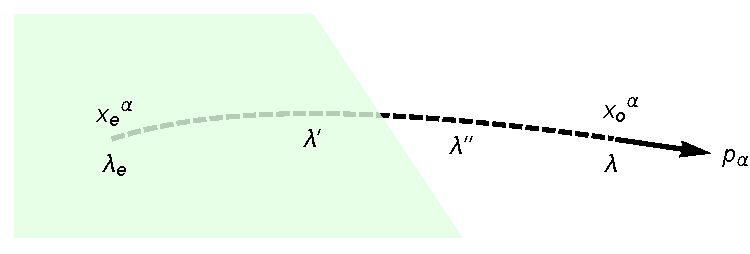
\includegraphics[width=\columnwidth]{affine_parameter_label}
  \caption{Affine parameterization of a neutrino trajectory of momentum
    $p_\alpha$.
    The fiducial observer with velocity $u^\alpha$ sits at $x^\alpha_o$,
    the neutrino emission event is at $x^\alpha_e$. The affine parameter
    increases from the emission event: $\lambda_e<\lambda'<\lambda''$.}
  \label{fig:affine_param}
\end{figure}

\subsection{The Rendering Equation}
\label{ssec:rendering_eqn}
Defining the source function
$\mathscr{S}^*\equiv\mathscr{E}^*/\mathscr{K}^*$,
we can integrate Eqn.~\ref{eqn:boltzmann_linear} directly,
\begin{equation}
  \label{eqn:rendering}
  f(\lambda) = f(\lambda_e) e^{-\tau(\lambda,\lambda_e)} +
  \int_{\lambda_e}^\lambda d\lambda'\,e^{-\tau(\lambda,\lambda')}
  \mathscr{K}^*(\lambda') \mathscr{S}^*(\lambda'),
\end{equation}
where the optical depth is defined,
\begin{equation}
  \label{eqn:optical_depth}
  \tau(\lambda,\lambda') \equiv -\int_{\lambda'}^\lambda
  d\lambda'' \, \mathscr{K}^*(\lambda''),
\end{equation}
and the parameterization conventions are depicted in
Fig.~\ref{fig:affine_param}.

\subsection{Neutrinosurface Approximation}
\label{ssec:neutrinosurface}
\todo{derive $\tau=2/3$ approx \cite[Chap.~4]{shu1991-book_radiation},
  and \cite{miln1921-radiative_equil_1}}
In the simplified configuration of a plane-parallel atmosphere, the
rendering equation reduces to 
\begin{equation}
\label{eqn:neutrinosurface}
  f(\lambda) = f^{\rm eq}(\lambda_e),
\end{equation}
where $\tau(\lambda,\lambda_e)=2/3$.
At an optical depth of $2/3$, the energy flux is equivalent to the
blackbody value $\sigma T^4$, with $\sigma$, the Stefan-Boltzmann radiation
constant.
\todo{verify}

\subsection{Moments of the Distribution Function}
\label{ssec:moments}
\todo{code these up}
We may take angular moments of the distribution function:
\begin{align}
  \label{eqn:J}
  J(\varepsilon) &=
  \varepsilon^3 \oint d\Omega' f(\varepsilon, \ell'_\beta) \\
  \label{eqn:Ha}
  H^\mu(\varepsilon) &=
  \varepsilon^3 \oint d\Omega' f(\varepsilon, \ell'_\beta) \ell^\mu \\
  \label{eqn:Sab}
  S^{\mu\gamma}(\varepsilon) &=
  \varepsilon^3 \oint d\Omega' f(\varepsilon, \ell'_\beta) \ell^\mu \ell^\gamma,
\end{align}
representing specific energy density, specific energy flux, and
specific momentum flux, respectively.
Here ``specific'' refers to the quantity being integrable over neutrino energy.
\todo{relate moments to other frames?}
Integrals~\ref{eqn:J}--\ref{eqn:Sab} are performed over a solid angle in
momentum space while holding $\varepsilon$ constant:
$d\Omega \equiv d(\cos\upsilon_1)\,d\upsilon_2$.
\todo{consistent with Eqn.~\ref{eqn:def_direction}?}

\subsection{Numerical Implementation}
\label{ssec:numerical}
Much of our numerical implementation is borrowed from the geodesic evolution
system described in~\cite{bohn2016-code}.
We integrate Eqns.~\ref{eqn:geodesic_x} and~\ref{eqn:geodesic_p} in the form given by
\citep{hugh1994-eh_finding}.
\todo{describe eqns for $f_{\rm integ}$ and $\tau$}
\todo{describe $\nu$-specific numerics}

\section{Code Tests}
\label{sec:tests}

\subsection{Dummy Tests}
[Maybe we don't need to present these tests, but make sure to establish
confidence in the basics:
gravitational redshift, Doppler shift, thermodynamic equilibrium.]
\todo{setup and run dummy tests}

\subsection{Homogenous Absorbing Star}
[Test described in~\cite[Sec.~3.2]{smit1997-two_moment}.]
\todo{Jerred: run test}

\subsection{Homogenous Scattering Star}
\todo{maybe drop this test}
[Test presented in~\cite{humm1971-grey_transfer}
and described in~\cite[Sec.~9.1.1]{abdi2012-monte_carlo}.
Our version would be a point source embedded in a spherical distribution
of purely elastic-scattering material. It requires an analytical estimate
of $J$.]
\todo{formulate analytic $J$.}

\subsection{Post-Bounce Neutron Core}
[Standard radiation transport test described in~\cite{ocon2015-gr1d_with_nu},
and in \cite[App.~E.6]{fouc2015-m1_nsbh},
and in~\cite{abdi2012-monte_carlo}.]
\todo{Evan: provide initial data and $H^r(\varepsilon)$}
\todo{Jerred: setup and run test}

\subsection{Disk Comparison to M1}
[Compute total and relative number and energy luminosities for a disk evolved
in one of~\cite{fouc2015-m1_nsbh, fouc2016-m1_nsns, fouc2016-m1_evolve_n}.
Expect agreement within factors of a few (?).]
\todo{code up moment integrals}
\todo{compute luminosities from M1}
\todo{compute luminosities from ray tracing}

\section{Applications}
\label{sec:applications}

\subsection{Emission Spectra}
\label{ssec:spectra}
The merger models are described in \cite{fouc2015-m1_nsbh, fouc2016-m1_nsns}.
[Something like this is presented in~\cite[Fig.~10-11]{pere2014-nu_wind};
compare.]
\todo{code up moment integrals}
\todo{compute $H^r(\theta;\varepsilon)$ in nsns and nsbh}
\todo{maybe compute at several times}

\subsection{Closure Relation}
\label{ssec:closure}
\todo{figure out your approach}
[This is a little tricky. Unless we can come up with a new improved analytic
closure relation and use ray tracing to evaluate its trustworthiness,
it's going to be hard to get anything useful from computing
$S^{\alpha\beta}$.]

[Maybe the variable Eddington closure is more suitable to this application.
If I understand it right, applying ray tracing to that method would require
computing $S^{\alpha\beta}$ on the fly throughout the spatial volume.
That would certainly be doable for a quasi-stationary disk configuration.]
\todo{compute $S^{\alpha\beta}$ and evaluate its effect on evolution}

% ******************************************************************************
\appendix

\section{Source Terms}
\label{sec:source_terms}
Here we present the sources comprising the right hand side of the
Boltzmann Equation (Eqn.~\ref{eqn:boltzmann}). The sources for the neutrino
distribution function $f(x^\alpha;p_\beta)$ arise from collision processes
producing, removing, or scattering to/from that point in phase space.
The weak interaction rates for each process involve integrals of
the neutrino distribution function $f(x^\alpha;p'_\beta)$ and that of the
antineutrino $\bar{f}(x^\alpha;p'_\beta)$ over a momentum volume
$dP'$ (Eqn.~\ref{eqn:dP}).

We follow
\cite{brue1985-core_collapse} and \cite[Sec.~4]{shib2011-truncated_moment}
by separating these processes into four categories:
\begin{equation}
  \label{eqn:four_sources}
  C[f] \equiv C_{\rm AE} + C_{\rm SE} + C_{\rm SI} + C_{\rm TP},
\end{equation}
representing charged-current absorption and emission, elastic scattering,
inelastic scattering, and thermal pair annihilation and production. Each term
is computed by summing the weak interaction rates of the processes from the
relevant category given in Tab.~\ref{tab:neutrino_processes}.
These rates are computed most easily as traditional emissivities and opacities
in the fluid frame of reference;
but since we use them in the form of an invariant emissivity and opacity
(defined e.g. in \ref{eqn:inv_emissivity} and \ref{eqn:inv_opacity},
and obeying Eqn.~\ref{eqn:boltzmann_linear})
they take the same numerical value in any frame of reference
and are completely independent of our choice of fiducial observer $u^\alpha$.
\todo{confirm}

Each source term is unique to the neutrino or antineutrino species modeled,
and consists of a sum over all of the processes contributing to that
category of interaction. For example:
$C^{\nu_e}_{{\rm AE}} = \sum_i\,C^{\nu_e}_{{\rm AE},i}$,
where $i$ labels the absorption/emission processes involving $\nu_e$
in Tab.~\ref{tab:neutrino_processes}.
By contrast $C^{\nu_x}_{{\rm AE}} = 0$,
where $\nu_x$ stands for any of the four heavy-lepton neutrinos and
antineutrinos.

We compute our rates using the open source neutrino interaction
library \lstinline{NuLib}~\footnote{\url{http://www.nulib.org}}.
We compile a table of sources defined over the four dimensions of
density, temperature, electron-fraction, and neutrino energy, and
interpolate quad-linearly to the points sampled along each ray.
\todo{derive and type up all sources in terms of $J$ and $H^\alpha$
  following \cite[Sec.~4]{shib2011-truncated_moment}}

\begin{table}%[h]
  \caption{
    We analyze neutrino interaction processes in terms of these categories.
    $\nu$ without a label represents a neutrino or antineutrino of any flavor,
    $N$ represents a nucleon $n$ or $p$,
    ${}^ZA$ represents a nucleus with mass number $A$ and charge $Z$, and
    $\gamma$ represents a high-energy photon.
    A prime indicates a change in that particle's energy.
  }
  \label{tab:neutrino_processes}
  \begin{tabularx}{\columnwidth}{X X}
    \hline \hline
    absorption/emission
    & $\nu_e + n \leftrightarrow e^- + p$                          \\
    & $\bar{\nu}_e + p \leftrightarrow e^+ + n$                    \\
    & $\nu_e + {}^AZ \leftrightarrow e^- + {}^A(Z+1)$              \\
    & $\bar{\nu}_e + {}^AZ \leftrightarrow e^+ + {}^A(Z-1)$        \\
    \hline
    elastic scattering
    & $\nu + N \leftrightarrow \nu + N$                            \\
    & $\nu + {}^AZ \leftrightarrow \nu + {}^AZ$                    \\
    \hline
    inelastic scattering
    & $\nu + e^- \leftrightarrow \nu' + e^{-'}$                    \\
    & $\nu + e^+ \leftrightarrow \nu' + e^{+'}$                    \\
    \hline
    thermal pair processes
    & $\nu + \bar{\nu} \leftrightarrow e^{-} + e^{+}$              \\
    & $\nu + \bar{\nu} + N + N \leftrightarrow N' + N'$            \\
    & $\nu + \bar{\nu} \leftrightarrow \gamma$                     \\
    \hline \hline
  \end{tabularx}
\end{table}

\subsection{Absorption and emission via charged current}
\label{ssec:sources_ae}
At neutrino and thermal energies well below $m_{\mu}\sim100\,{\rm MeV}$
only charged current processes involving $\nu_e$ and $\bar{\nu}_e$ are allowed.
For each of these processes, $i$, we may write an emission and absorption
coefficient as a function of the interaction cross-section
(e.g. \cite[Eqn.~A5]{brue1985-core_collapse}):
\todo{explain Fermi-blocking}
\begin{align}
  \label{eqn:sources_ae_1}
  C_{{\rm AE},i}
  &= \mathscr{E}_{{\rm AE},i} (1-f) - \mathscr{K}_{{\rm AE},i} f \\
  \label{eqn:sources_ae_2}
  &= \mathscr{E}_{{\rm AE},i} - (\mathscr{E}_{{\rm AE},i} + \mathscr{K}_{{\rm AE},i}) f,
\end{align}
with
\begin{equation}
  \label{eqn:inv_emissivity}
  \mathscr{E}_{{\rm AE},i} = \frac{(2\pi)^3}{\varepsilon^2}\eta_{i},
\end{equation}
where $\eta$ is the traditional emissivity with dimension
$[\eta]={\rm energy}\,{\rm length}^{-3}\,{\rm time}^{-1}\,{\rm energy}^{-1}\,{\rm steradian}^{-1}$,
and
\begin{equation}
  \label{eqn:inv_opacity}
  \mathscr{K}_{{\rm AE},i} = \varepsilon \chi_i,
\end{equation}
where $\chi$ is the traditional opacity with dimension
$[\chi]={\rm length}^{-1}$.

\subsection{Elastic scattering}
\label{ssec:sources_es}
Neutrino scattering on particles of mass much greater than $\varepsilon$
is essentially iso-energetic
(e.g. \cite[Eqn.~A8]{brue1985-core_collapse}).
\begin{equation}
  \label{eqn:sources_es}
  C_{{\rm SE},i}
  = \mathscr{K}_{{\rm SE},i} \Phi_{{\rm SE},i} - \mathscr{K}_{{\rm SE},i} f,
\end{equation}
with
\begin{align}
  \label{eqn:es_factor}
  \Phi_{{\rm SE},i} &\equiv \frac{\varepsilon^3}{\mathscr{K}_{{\rm SE},i}}
  \oint d\Omega' R(\ell_\alpha,\ell'_\beta)f(\ell'_\beta) \\
  \label{eqn:es_opacity}
  \mathscr{K}_{{\rm SE},i} &\equiv \varepsilon^3
  \oint d\Omega' R(\ell_\alpha,\ell'_\beta),
\end{align}
where $R(\ell_\alpha,\ell'_\beta)$ is the scattering kernel from direction
$\ell'_\beta$ to direction $\ell_\alpha$
having dimension $[R]={\rm energy}^{-1}$.

\subsection{Inelastic scattering}
\label{ssec:sources_is}
(e.g. \cite[Eqn.~A6]{brue1985-core_collapse}).

\subsection{Thermal pair annihilation and production}
\label{ssec:sources_pp}
(e.g. \cite[Eqn.~A9]{brue1985-core_collapse}).

% ******************************************************************************
\bibliography{references}

\end{document}
